\documentclass[a4paper, 11pt, finnish]{article}
\usepackage{graphicx}
\usepackage{ucs}
\usepackage[utf8x]{inputenc}
\usepackage[T1]{fontenc}
\usepackage[finnish]{babel}

\setlength{\parindent}{0pt}
\setlength{\parskip}{1ex plus 0.5ex minus 0.2ex}

\author{Topi Talvitie}
\title{turrIDEvelop: Käyttöliittymä}

\begin{document}
\maketitle

\section{Navigaatiorakenne}
\begin{centering}
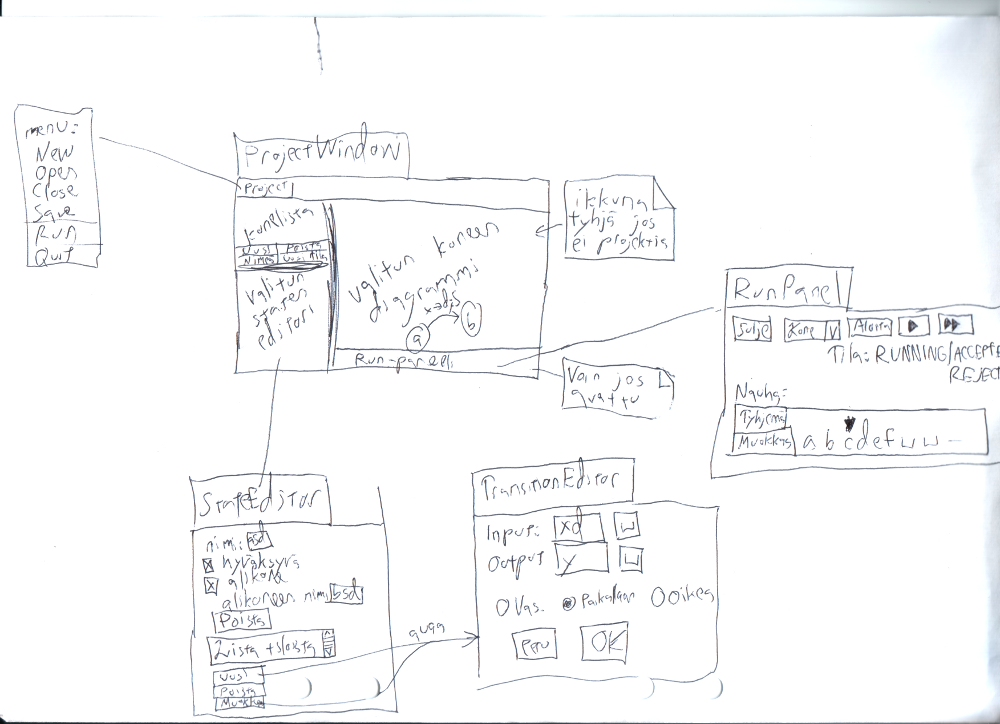
\includegraphics[width=14cm]{navigaatio.png}
\end{centering}

\section{Käyttöliittymän toteutus}
Kaikkien elementtien juurena toimii ProjectWindowin hallinoima JFrame, joka
hoitaa projektien avaamisen, tallentamisen ja sulkemisen. Se myös ylläpitää
konelistaa ja kun kone valitaan, avaa MachineViewin siihen. Kun MachineViewistä
valitaan tila, se ilmoittaa siitä ProjectWindowille joka avaa sen StateEditorin
vasempaan palkkiin. ProjectWindow hallinnoi myös RunPanelia ja sen sulkemista.

MachineView piirtää valitun koneen tilat ja siirtymät ja mahdollistaa tilojen
valitsemisen ja siirtelyn. MachineView tarjoaa myös mahdollisuuden siirtyä
tilanvalintatilaan missä valittu tila annetaan valitulle
StateChoiceHandlerille. StateEditor käyttää tätä ominaisuutta siirtymän kohteen
valinnassa.

StateEditorissa voidaan muokata tilan tietoja ja tilasiirtymiä. Se raportoi
muutokset MachineViewille johon se liittyy, jotta muutokset näkyvät heti. Tilan
luomisessa ja muokkaamisessa se avaa TransitionEditor-dialogin siirtymän
tietojen muokkaamiseen.
\end{document}
